\chapter{Overview and methods}
\label{chap:overwiev} % id kapitoly pre prikaz ref
In this chapter, we describe basic concept of artificial models called neural networks. We will breafly explain different aproaches of training such models to perform specific task and we will explain some examples of models that are designed to each type of training approaches.

\section{Neural networks} \label{sec:nn}

Neural networks are artificial inteligence models with applications in many domains, such as forecasting, computer vision or natural language processing. Since these models are successful, but still has some limitations in performance, it  is useful to study them and try new approaches, that could possibly achieve better results.

Neural network is composed of processing units called neurons, which are connected to layers. Layers are then connected to network. Each neuron has input features, and internal weights, which are used for computation of weighted sum. Result of weighted sum is scalar and it is transformed by function, called activation function. Most used activation functions are logistic function, hyperbolic tangent or rectified linear unit - mostly in deep networks, with many layers.

\section{Convolutional neural networks}
Convolutional neural networks (CNNs) are a specialized kind of neural network for processing data
that has a known grid-like topology, for example image data (2-D grid of pixels).
CNNs have special type of layers - convolutional layers. These layers do not consist of neurons, but matrices of weights called kernels or filters. Each layer has it`s own trainable weights and provides specialized kind of linear operation - convolution. We can see this process described in figure \ref{fig:convo}. Convolution leverages important ideas, such as sparse interactions or parameter sharing that can help improve a machine learning system. Another operation, called pooling, is also often emplyed in CNNs. When pooling layers are employed, network can be invariant to augmentations, such as translation, rotation or scaling. \cite{Goodfellow-et-al-2016} 

\begin{figure}
    \centering
    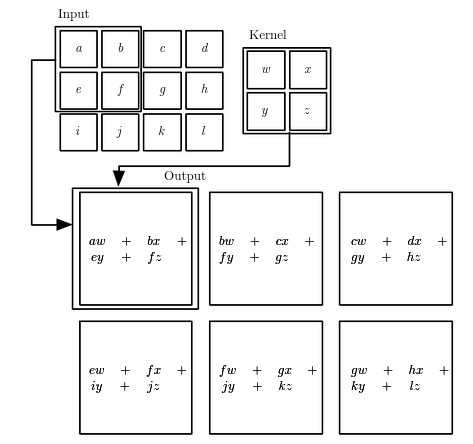
\includegraphics[width=0.7\textwidth]{figs/convo.png}
    \caption{Convolution in CNNs \cite{Goodfellow-et-al-2016}}
    \label{fig:convo}
\end{figure}

\section{Supervised models}

Recently, one of most used method for achieving useful real world results with neural network models is using supervised learning. It is simply mapping input described by set of features to output labels. In the beggining, mapping is not very accurate, so the aim of training is to adjust models parameters, called weights, such that the inference is more correct then before adjustment.

\subsection{Multi layer perceptron}
We already introduced neural networks in section \ref{sec:nn}. Multi layer perceptron (MLP) is neural network with input layer, output layer and at least one hidden layer. The goal of a MLP is to approximate some function $f^*$ by samples from this function. Samples are pairs of input and output $(x, y)$. MLP defines mapping $y = f^*(x, \theta)$, where $\theta$ denotes parameters of the model - weights. At the beginning, weight are randomized. Then using supervised learning from training examples, weights are adjusted to minimize loss function, which is expression of prediction error. For training of MLP, error backpropagation algorithm is used. \cite{Goodfellow-et-al-2016}


\section{Unsupervised models}

Unsupervised models work with data, that consist of only input samples, which means they does not have assigned desired output. This is common case, when we have some new task on real world data, that we do not know the desired output. Unsupervised mode
They are able to capture the similarities of data or unseen data structures. Examples of such neural model is the Self-organizing map.

\subsection{Self-organizing map}
\label{sec:som}

The self-organizing map (SOM), originally proposed by Kohonen in 1990 \cite{kohonen1990}, is unsupervised neural model, based on competitive and cooperative principles. It is mostly used for clustering and visualization of high-dimensional data onto a low-dimensional grid. The grid is composed of units - neurons, each one associated with a prototype vector from the original data space. The learning algorithm enforces a topology constraint, so that neighboring map units correspond to prototypes that are close in the original space, according to euclidean distance. \cite{desom2019} 

\begin{figure}[h!]
    \centering
    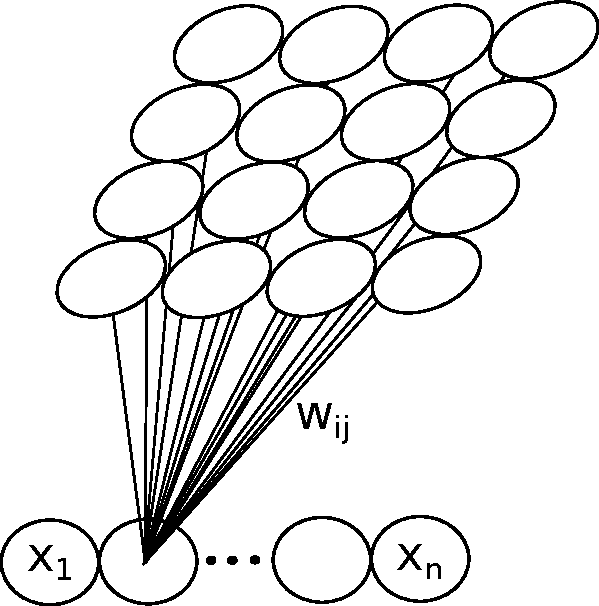
\includegraphics[width=0.4\textwidth]{figs/som.pdf}
    \caption[Self-organizing map]{In the bottom of the image, there is n-dimensional input vector. In the upper part, there are neurons of the Self-organizing map ordered in grid-like structure. In the middle part, there are weights of the network. Each item of input vector has weighted connection with each neuron. Figure is from \cite{rebrova2013}.}
    \label{fig:som}
\end{figure}

In process of training, competitive principle is used first. Among all neurons in network, one denoted $i^*$ (winner neuron, prototype) is chosen by equation \ref{eq:somwin}. It is the one closest to the input $x$. As a distance measure, Euclidian norm is used.
\begin{equation}
	\label{eq:somwin}
	i^* = {\argmin}_i \|{x}(t)-{w}_i\|
\end{equation}

Then all weights are adjusted based on cooperative principle. The change of each weight is computed by equation \ref{eq:somlearn}. The neurons closest (in low dimensional grid) to winner are adjusted more, than those farther from it. That means all neurons are moved to  represent input $x$ better. The magnitude of change is defined by learning rate $\alpha(t)$ decreasing in time. Distance of neurons in grid is defined by neighbourhood function denoted as $h$. Commonly used neighbourhood functions are Manhattan distance (eq. \ref{eq:manhatdist}) or Gausian distance (eq. \ref{eq:gaussdist}). 
\begin{equation}
	\label{eq:somlearn}
	\Delta{w}_i = \alpha(t) h(i,i^*) ({x}(t)-{w}_i),
\end{equation}


\begin{equation}
	\label{eq:gaussdist}
	h(i,i^*) = e^{-d(i,i^*)^2/{\sigma}^2(t)}
\end{equation}

\begin{equation}
	\label{eq:manhatdist}
	h(i,i^*) = \begin{cases}
		1  & \mbox{if } d_M(i,i^*)\le{\lambda}(t) \\
		0  & \mbox{if } \text{otherwise}%d_M(i,i^*)>{\lambda}(t)
	\end{cases}
\end{equation}

\subsection{SOM evaluation methods}
For evaluation of SOM performance during the training, three metrics are typically used - quantization error, winner discrimination and entropy. Descriptions and equations of metrices are from \cite{rebrova2013} and \cite{vanco2010-som}.

\subsubsection{Quantization error}
Quantization error (QE) calculates the average error at the unit as a result of quantization process. It is calculated as mean of mean squared errors (MSE) of difference of $k$-th input $x^k(t)$ and its winner $i^*$ (eq. \ref{eq:qe}), where $M$ denotes number of inputs and $N$ denotes their dimensionality. Well trained SOM should have small quantization error.

\begin{equation}
	\label{eq:qe}
	QE = \frac{1}{M} \sum_{k=1}^M MSE(x^k(t) - i^*) %% = \frac{1}{M} \sum_{k=1}^M \frac{1}{N} \sum_j^N (x^k_j(t)  - i^*_j)^2
\end{equation}

\subsubsection{Winner discrimination}
Winner discrimination (WD) is proportion of neurons chosen as winners during training. We can denote set of all neurons as $\mathcal{A}$ and $t$ stands for any moment during training, so $i^*(t)$ is winner chosen in moment $t$. Then WD is computed as in equation \ref{eq:wd}. Well trained SOM should choose all or almost all neurons as winners.

\begin{equation}
	\label{eq:wd}
	WD = \frac{|j | \exists t : j = i^*(t)|}{|\mathcal{A}|}
\end{equation}

\subsubsection{Entropy}
Entropy (E) is a measure of order in the system. Entropy for SOM evaluates how often various units become winners, so the highest entropy means most balanced unit participation in the competition process. Computation of entropy is shown in equation \ref{eq:e}, where $p$ denotes vector, which contains probability of each unit to be chosen. Probability is estimated from training as a number of usages of a unit devided by all unit usages.

\begin{equation}
	\label{eq:e}
	E = - \sum_i (p_i  \log_2{p_i})
\end{equation}

\section{Semi-supervised models}

Semi-supervised learning combines supervised approach with unsupervised. Unsupervised learning is usualy used for solving an auxilary task (for example denoising), that helps supervised learning. Unsupervised approach can be used in pretraining or alongside with supervised learning, which is more effective way. In this case, role of unsupervised learning is to find new features which correlate with the features selected by supervised learning, not pushing new independant features to the representation intended for supervised learning, even if these features carry information about the inputs. \cite{valpola2015}

Semi-supervised learning use unlabeled data to improve model's learning possibilities. Usually, creating huge labeled dataset is difficult, but collecting huge amount of unlabeled and smaller portion of labeled data is feasible. This is, why Semi-supervised models can be really usefull and worth studying. Most Semi-supervised models are based on two ideas - consistency regularization and pseudo labels. 


\subsection{Consistency regularization models}

Consistency regularization is concept which use unlabeled datapoint which is augmented in two different ways. The augmentations do not change the label. Then both augmented data are used as input of neural model and consistency of these data predictions is enforced. Usually model is updated in such manner that new predictions on two augmentations are more similar. There are many Semi-supervised models based on consistency regularization method, such as Ladder Networks, Pi-Model, Temporal Ensembling or Siamese neural network.

\subsubsection{Ladder Network}

Concept of Ladder Network was originaly introduced by Harri Vapola \cite{valpola2015}. 
The auxilary task of this model is to denoise representations at every level of the autoencoder using skip connections from the encoder to the decoder part. The skip connections relieve the pressure
to represent details at the higher layers of the model because, through the skip connections, the
decoder can recover any details discarded by the encoder. \cite{Rasmus2015} 

Difference between standard autoencoder and Ladder network with skip connections is shown in figure \ref{fig:ladder}.

\begin{figure}[h!]
    \centering
    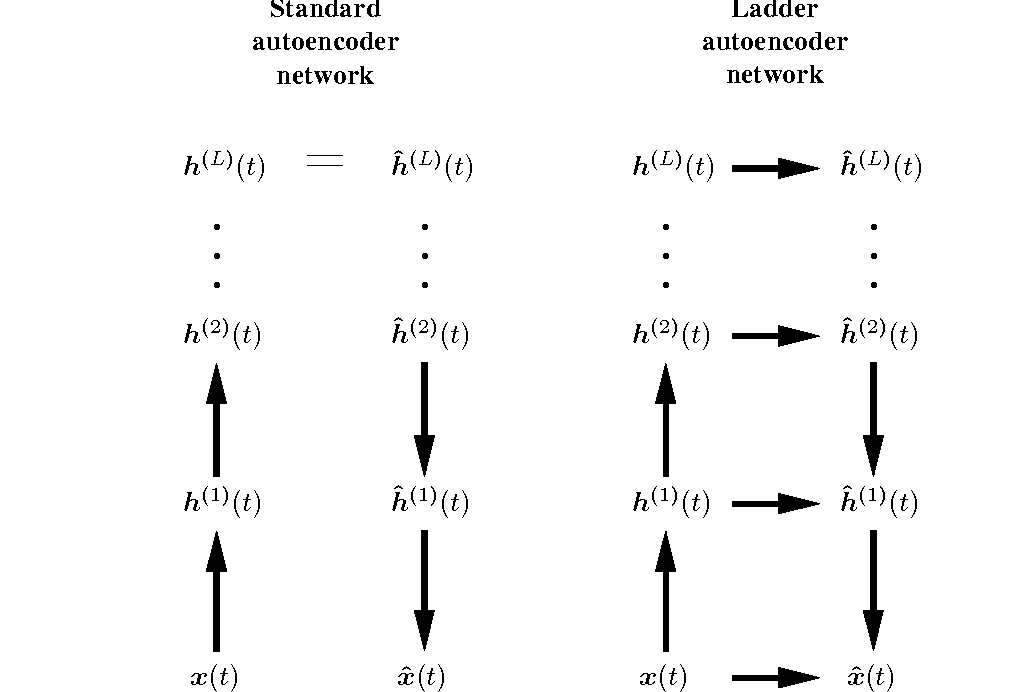
\includegraphics[width=1\textwidth]{figs/ladder.png}
    \caption{Autoencoder and Ladder network models \cite{valpola2015} }
    \label{fig:ladder}
\end{figure}

Rasmus et al. \cite{Rasmus2015} introduced new way of usage of the Ladder network in Semi-supervised learning. The network use original and augmented input. It makes predictions for both using two neural paths. It enforces consistency between predictions using consistency cost. For labeled datapoints, classification cost is applied. The enhanced versions of Ladder networks use also denoising function that takes the feature vector from particular layer of perturbed
path of the network and reconstructs the feature vector from the corresponding layer of the unperturbed path. \cite{tuna}

\subsubsection{Pi-Model and Temporal Ensembling}
Pi-Model and Temporal Ensembling were introduced in the same article by Laine et Aila \cite{laine2017}. Their approach self-ensembling, that means forming ensemble predictions during training. They use outputs of single supervised model under different training conditions (different training epoch, regularization, augmentation), as ensemble prediction.

\begin{figure}[h!]
    \centering
    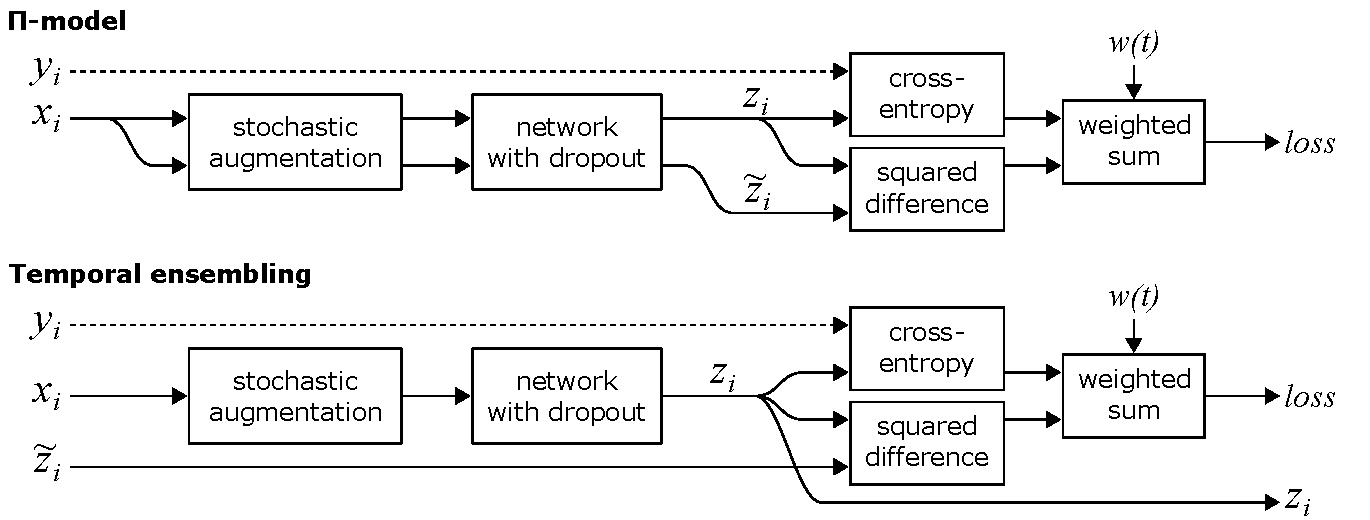
\includegraphics[width = 1\textwidth]{figs/pi-tempens.pdf}
    \caption{Pi-model and Temporal ensembling model \cite{laine2017}}
    \label{fig:pi-tempens}
\end{figure}

\textbf{Pi-model} described in upper part of figure \ref{fig:pi-tempens} uses two different data perturbations (Gaussian noise, random translation) on the same datapoint. Then two different dropout conditions are used in forward pass of the input. The outputs of forward passes are denoted $z$ and $\Tilde{z}$. In case of labeled datapoint, supervised cost of $z$ and desired output $y$ is computed as cross-entropy. Also unsupervised cost, squared difference of $z$ and $\Tilde{z}$ is computed. These cost functions are combined together using loss weightening function $w(t)$ which ramps up during training.

\textbf{Temporal Ensembling} model is similar to Pi-model. It is displayed in the bottom part of figure \ref{fig:pi-tempens}. It uses the same cost functions as Pi-model, but the way it makes self-ensembling is different. Temporal Ensembling ensambles network predictions over multiple previous training epochs. For $i-th$ input, it makes one augmented datapoint and one network prediction $z_i$. This prediction is used to compute $\Tilde{z_i}$ for following epoch and for computation of supervised and unsupervised costs. 
For compuation of $\Tilde{z_i}$ accumulated prediction vector $Z$ is also used. In this vector we store information about previous predictions, the newest has the highest impact on the output $Z$ and the oldest are slowly being forgotten. Bellow are displayed formulas for computation of $\Tilde{z_i}$:

\begin{equation}
    Z = \alpha Z + (1 - \alpha) z
\end{equation}

\begin{equation}
        \Tilde{z} = \frac{Z}{1 - \alpha^t}
\end{equation}

\newpage
\subsubsection{Siamese neural network}
Siamese neural network (SNN) by Bromley et al. \cite{bromley1993} is network suitable for dataset which consist of pairs. It is composed of two subnetworks with shared set of weights which are not connected one to anoter, but both are connected to common hidden layer, which produces one common output. This output is an estimate of semantic distance of the pair. The architecture of SNN is shown in figure \ref{fig:siamese}.


\begin{figure}[h!]
    \centering
    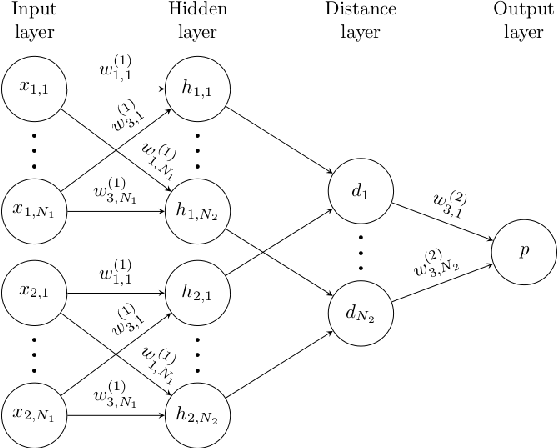
\includegraphics[width=0.7\textwidth]{figs/siamese.png}
    \caption{Siamese neural network \cite{Koch2015SiameseNN}}
    \label{fig:siamese}
\end{figure}


\subsection{Models using pseudo-labels}
Pseudo-label methods aim to assign labels to unlabeled part of dataset. Pseudo-labeling was described by Lee \cite{lee2013}. He proposed to train neural network on labeled and unlabeled data simultaniously. Pseudo-labels for unlabeled data are picked as class with maximum predicted probability (one-hot vector). Loss for both labeled and unlabeled samples is computed as cross-entropy of prediction and one-hot label or pseudo-label vector.

This idea work good but has some problems such as lack of consideration of any prior knowladge about the visual similarity of classes. To resolve this problem, Nassar et al. \cite{nassar} created model called SemCo. 

\subsubsection{SemCo}
SemCo model is based on pseudo-labeling method, consistency regularization and co-training ideas. Co-training means training two models, classifiers, with different views of the data, where each model is trained on the other’s most confident predictions. SemCo uses two different views of the label - regular one-hot view and distributed view, coresponding to two classifiers - one-hot classifier and semantic supervised classifier. Those classifiers produce two types of losses - supervised and unsupevised, based on type of training sample. Another part of total loss is Co-training loss, which enable classifiers to learn from each other. \cite{nassar}


\begin{figure}[h!]
    \centering
    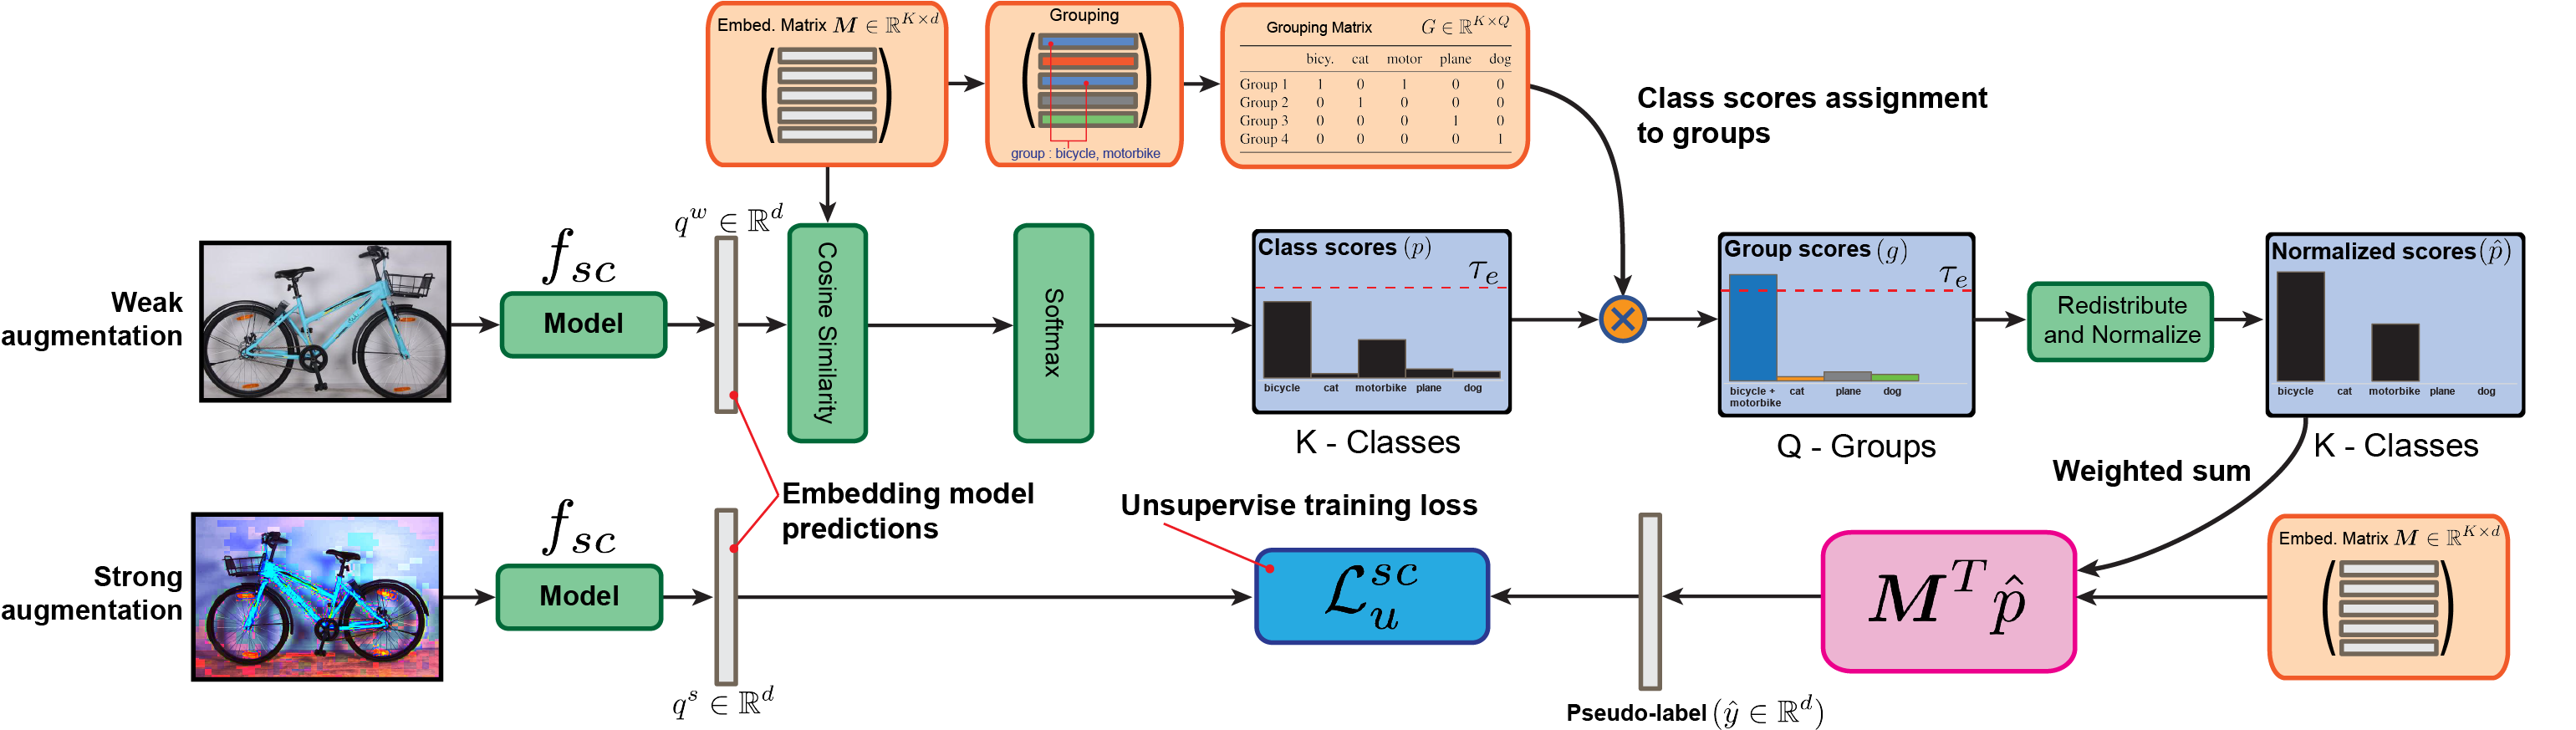
\includegraphics[width=1\linewidth]{figs/semco_unlabelled_loss_precedure.png}
    \caption{SemCo model : unsupervised cost computation in semantic classifier \cite{nassar}}
    \label{fig:semco}
\end{figure}

Semantic classifier supervised cost $\mathcal{L}^{sc}_s$ minimizes cosine loss between the true label and predicted label. One-hot supervised cost $\mathcal{L}^{oh}_s$ uses cross-entropy instead of cosine loss. 
For unsupervised cost from semantic classifier $\mathcal{L}^{sc}_u$, it uses weakly and strongly augmented input. Output of network for weakly augmented input is pseudo-label for strongly augmented input. It also take into account, that some classes are semantically similar, so it uses technique of label-grouping. In label-grouping for example bicycles and motorcycles form one group together, because objects are similar. Previous probabilities of classes are recomputed using grouping matrix. This helps create better pseudo-labels based on knowledge about classes present in dataset. This process is shown in figure \ref{fig:semco}. In One-hot classifier, for computation of unsupervised cost $\mathcal{L}^{oh}_u$ label grouping is not used. Total loss is computed as weighted sum of described costs, as described in \ref{eq:semco-loss}, where $\lambda_u $ and $\lambda_{co}$ are fixed parameters. \cite{nassar} 


\begin{equation}
    \mathcal{L}_{total} = \mathcal{L}^{sc}_s + \mathcal{L}^{oh}_s + \lambda_u (\mathcal{L}^{sc}_u + \mathcal{L}^{oh}_u) + \lambda_{co} \mathcal{L}_{co}
    \label{eq:semco-loss}
\end{equation}


\subsection{Mean Teacher model}
\label{mtm-chapter}
The Mean Teacher model (MT) proposed by Tarvainen et al.\cite{tarvainen} is also example of consistency regularization model. Consistency regularization is provided by using consistency cost \ref{eq:mt-loss-unsup}. MT consists of two deep convolutional neural networks with the same layer architecture. Each network has its own trainable weights. First network is called student and its weights are denoted $\theta$, second is called teacher, with weights $\theta^\prime$. Mean Teacher is intended for classification problem.
During training, model use both, labeled and unlabeled data. Labeled data have assigned desired output (label), while unlabeled data are from the same domain of classes, but they has no label. 

Important part of model training is using augmentations, for example translation, rotation, addition of small noise etc. Each datapoint, usually image, is augmented in two different ways. One augmented image is then used as input for student network, the other for teacher network. Augmentation technique is commonly used as it improves results mostly in supervised learning. %% \cite{krizhevsky2012}.

Training method of student model differs from teachers training rule. Student's weights are updated using backpropagation, teacher uses  Exponential moving average (EMA) of weights of student model. EMA rule can be written as equation \ref{eq:ema}, where 
$\theta^\prime_t$ is teachers weight matrix in time $t$ and $\theta_{t}$ is students weight matrix in time $t$ and $\alpha$ is hyperparameter - learning rate. This strategy is called Temporal ensembling \cite{laine2016} and it represents composition of weights in different times, which is type of regularization.

\begin{equation}
    \theta_t^\prime = \alpha\theta^\prime_{t-1} + (1-\alpha)\theta_t
    \label{eq:ema}
\end{equation} 


Student's loss function consists of consistency cost and supervised cost of the model. 
Supervised cost $S(\theta)$ is calculated for student model as cross entropy of predictions for input $x_j$, augmented by augmentation $\eta$ and desired label $y_j$ only for labeled samples(equation \ref{eq:mt-loss-super}). Consistency cost  $J(\theta)$ is the expected distance between the prediction of the student model and the prediction of the teacher model (equation \ref{eq:mt-loss-unsup})  It is computed as Mean squared error (MSE) of difference in teacher and student predictions on the same input $x_j$ and different augmentations $\eta$ and $\eta^\prime$. This loss function does not use any labels for input data, therefore it is example of unsupervised learning and we can aply it on unlabeled data as well as on labeled data. 

\begin{equation}
	S(\theta) = \frac{1}{m} \sum_j^m \left[ -\log~P_f(y_j | x_j; \theta,\eta) \right]
	\label{eq:mt-loss-super}
\end{equation} 

\begin{equation}
	J(\theta) = \frac{1}{n} \sum_i^n {\| f(x_i,\theta^{\prime},\eta^{\prime}) - f(x_i,\theta,\eta) \|}^2
	\label{eq:mt-loss-unsup}
\end{equation} 

\noindent Total loss is then computed as weighted sum of $S(\theta)$ and $J(\theta)$, as shown in equation \ref{eq:mt-loss-sum}. Parameter $w_t$ is weight of consistency loss in time $t$. It's value slowly increases in time. Based on this loss function, student model is trained using error back-propagation algorithm and gradient descent.
The Mean Teacher model and training process is described in figure \ref{mtm}.

\begin{equation}
	Loss(\theta) = S(\theta) + w_t J(\theta),
	\label{eq:mt-loss-sum}
\end{equation} 



\begin{figure}[h!]
    \centering
    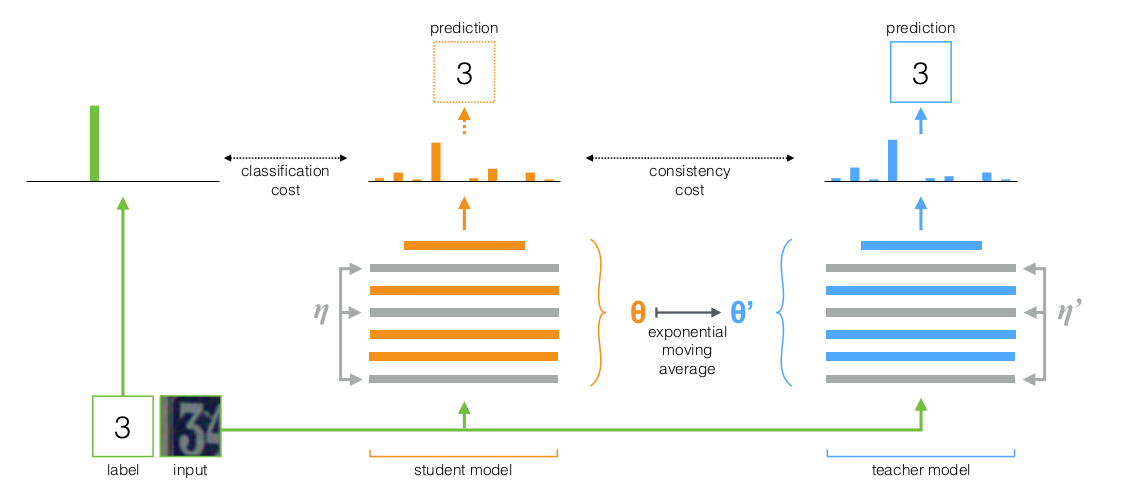
\includegraphics[width=1\textwidth]{figs/mt.png}
    \caption{Mean Teacher model}
    \label{mtm}
\end{figure}


\subsection{Binary mean teacher model}
\label{bmt}
Binary mean teacher model (BMT) is derived from previously described Mean Teacher model. Binary Mean Teacher was introduced by Tuna et al.\cite{tuna-bmt} and worked well for binary clasification whether the image contains containing wearable object (backpack) or not. BMT is described in figure \ref{fig:bmt}.

\begin{figure}[ht]
    \centering
    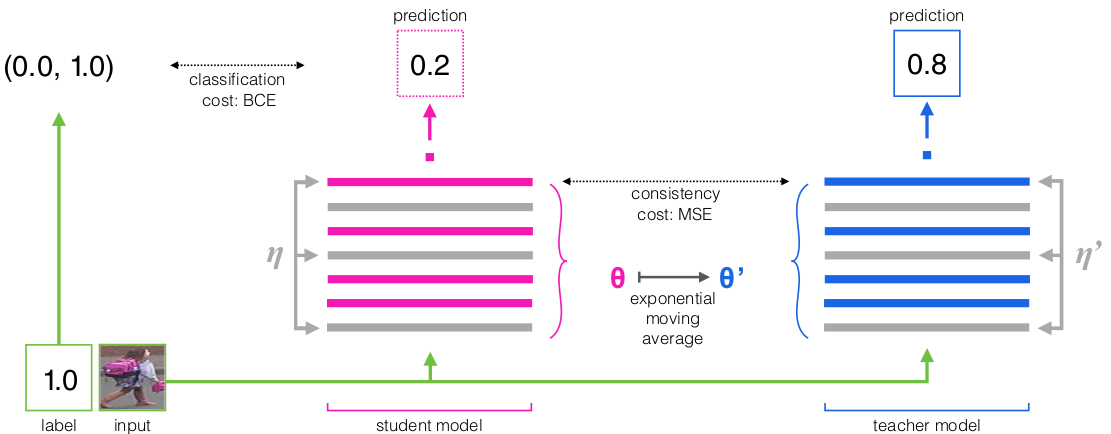
\includegraphics[width=1\textwidth]{figs/bmt.png}
    \caption{Binary mean teacher model}
    \label{fig:bmt}
\end{figure}


There are several changes in comparison to Mean Teacher model. 
Firstly, inferences of student's and teacher's network are only scalars, so they are not suitable for consistency loss. They are replaced by feature vectors produced by last convolutional layer. Another difference is, since the output is scalar, supervised cost which in MT is computed as Cross entropy is in BMT computed as Binary cross entropy (BCE). Supervised loss is shown in equation \ref{eq:bmt-sup}, consistency loss is shown in equation \ref{eq:bmt-unsup}. In consistency loss we denote weights from convolutional layers $\tau$. We can not use original notation $\theta$, because it denotes all weights (also those in fully connected layers). We can say $\tau \subset \theta$ and $\tau^{\prime} \subset \theta^{\prime}$. Inference in convolutional part is denoted by function $g$. Last change is in activation function of the last fully connected layer. In MT, softmax function was used. In BMT authors proposed sigmoid activation function. Total loss (eq. \ref{eq:bmt-loss-sum}) is computed similarly to MT model.


\begin{equation}
	S(\theta) = - \sum_{i}^{n}[y_j \log{\hat{y_j}} + (1-y_j)\log{(1-\hat{y_j})}]
	\label{eq:bmt-sup}
\end{equation} 

\begin{equation}
    J(\tau) = \frac{1}{n} \sum_i^n {\| g(x_i,\tau^{\prime},\eta^{\prime}) - g(x_i,\tau,\eta) \|}^2
	\label{eq:bmt-unsup}
\end{equation} 

\begin{equation}
	Loss(\theta) = S(\theta) + w_t J(\tau),
	\label{eq:bmt-loss-sum}
\end{equation} 

\subsection{Comparison of Semi-supervised models}

Results in following table \ref{tab:comparison} shows image classification of standard color image dataset CIFAR-10 into 10 classes using described models. All models, excluding $\Gamma$-model, use input augmentations.

\begin{table}[h!]
\centering
\begin{tabular}{|l|ll|l|}
\hline
                                & \multicolumn{2}{l|}{\textbf{CIFAR 10}}  & Source \\ \hline
\textbf{Total labelled samples} & \multicolumn{1}{l|}{\textbf{250}} & \textbf{4000} & \\ \hline
$\Gamma$-model (simple Ladder network) & \multicolumn{1}{l|}{-}&$20.40 \pm 0.47$&  \cite{Rasmus2015} \\ \hline
Pi model                        & \multicolumn{1}{l|}{-}& $12.36 \pm 0.31$& \cite{miyato2018virtual}\\ \hline
Temporal ensembling             & \multicolumn{1}{l|}{-}             & $12.16 \pm 0.24$  & \cite{miyato2018virtual}\\ \hline
Mean Teacher                    & \multicolumn{1}{l|}{$32.32 \pm 2.30$}&$6.28 \pm 0.15$ &\cite{nassar}, \cite{tarvainen} \\ \hline
Binary mean teacher             & \multicolumn{1}{l|}{-}& - &              \\ \hline
Siamese neural network          & \multicolumn{1}{l|}{-} & - &             \\ \hline
Pseudo-labeling                 & \multicolumn{1}{l|}{$49.78 \pm 0.43$}&$16.09 \pm 0.28$ & \cite{nassar} \\ \hline
SemCo & \multicolumn{1}{l|}{$5.12 \pm 0.27$}&$3.80 \pm 0.08$&\cite{nassar} \\ \hline
\end{tabular}
\caption{Comparison of Semi-supervised models}
\label{tab:comparison}
\end{table}